\chapter{Brückenkapitel (0)}
Im ersten Kapitel, oder eher im nullten gemäss Aufgabenbuch, repetieren wir einige Dinge, die ihr auf der Oberstufe gelernt habt.
Damit sind wir dann alle auf dem gleichen Stand.
Und teilweise erweitern wir unser Wissen bereits etwas, führen vielleicht neue Schreibweisen ein, formulieren die Rechengesetze evtl. etwas allgemeiner oder manchmal abstrakter, als du es bisher gewohnt warst. Vielleicht ist das für dich zum grössten Teil ein alter Hut - aber Übung macht den Meister!

\section{Rechnen mit Zahlen -- Die Rechengesetze}
Ein Gesetz ist bekanntermaßen eine feste Regel oder eine verbindliche Vorschrift.
An ihm darf man nichts rütteln oder verschieben, sondern man muss sich daran halten.
Genauso, wie es in den Gesetzbüchern Gesetze gibt, gibt es auch in der Mathematik Regeln, die gelten und beim Rechnen eingehalten werden müssen.
Diese sind die Rechengesetze oder Rechenregeln.
\begin{defn}{Rechengesetz}
		Ein Rechengesetz ist eine verbindliche Rechenvorschrift.
\end{defn}
Wenn du ein Rechengesetz missachtest, bekommst du natürlich keine Strafe von der Polizei.
Aber wenn du dich nicht an die Rechengesetze hältst, dann wird dein Ergebnis mit grosser Wahrscheinlichkeit falsch sein.
Die Rechengesetze gibt es also nicht, um verzweifelte Schüler:innen zu quälen, sondern sie ergeben mathematisch und logisch Sinn.

Wenn man von den Rechengesetzen spricht, dann meint man meistens das Assoziativgesetz, das Kommutativgesetz und das Distributivgesetz.
Sie sind die drei wichtigsten Rechengesetze.Wenn man den Begriff aber etwas weiter fasst, gibt es noch einige weitere Rechenregeln.
Diese sind etwa die Regel Punkt-vor-Strich, die Potenzgesetze und die Wurzelgesetze, oder Vorgehensweisen zum Auflösen von Klammern.
Fangen wir also an.

\subsection{Rechengesetze}

\begin{law}{Rechengesetze}
	\begin{enumerate}
        \item
			Kommen Potenzen vor, müssen diese als erstes berechnet werden.
		\item
			Klammern in Termen müssen zuerst aufgelöst werden. ("`von innen nach aussen"')
        \item
			Punktrechnungen ( $\cdot$ und : ) müssen vor Strichrechnungen ( + und -- ) ausgeführt werden.
		\item
			Assoziativgesetz der Addition:\\
			Für alle rellen Zahlen $a$, $b$ und $c$ gilt: $(a+b)+c = a+(b+c)$
		\item
			Assoziativgesetz der Multiplikation:\\
			Für alle rellen Zahlen $a$, $b$ und $c$ gilt: $(a\cdot b)\cdot c = a\cdot (b\cdot c)$
		\item
			Kommutativgesetz der Addition:\\
			Für alle rellen Zahlen $a$ und $b$ gilt: $a+ b= b+ a$
		\item
			Kommutativgesetz der Multiplikation:\\
			Für alle rellen Zahlen $a$ und $b$ gilt: $a\cdot b= b\cdot a$
		\item
			Distributivgesetz der Multiplikation:\\
			Für alle rellen Zahlen $a$, $b$ und $c$ gilt: $(a\pm b)\cdot c = a\cdot c \pm b\cdot c$
		\item
			Distributivgesetz der Division:\\
			Für alle rellen Zahlen $a$, $b$ und $c$ gilt: $(a\pm b): c = a: c \pm b: c$	
	\end{enumerate}
\end{law}

\begin{example}
Im folgenden Term darf nicht einfach von links nach rechts gerechnet werden, sondern es muss zuerst das Produkt berechnet werden:
\[
	5+5\cdot 3
\]
\end{example}

\begin{example}
Berechne den folgenden Term:
\[
	4\cdot(27-(3\cdot (5+3)+2))
\]
\end{example}

\begin{example}
Rechne vorteilhaft:
\[
	85+33+67
\]
\end{example}

\begin{example}
Rechne vorteilhaft:
\[
	7\cdot 4 \cdot 45
\]
\end{example}

\begin{example}
Ebenso:
\[
	24+33+76
\]
\end{example}

\begin{example}
Multipliziere aus:
\[
	4\cdot (20-5)
\]
\end{example}

\begin{example}
Manchmal bringt ausklammern einen Vorteil!
\[
	14\cdot 13 - 4\cdot 13
\]
\end{example}

\subsection{Primfaktoren, ggT und kgV}
Sowohl der Zahlentheorie als auch in der Bruchrechnung spielen Primfaktoren, grösste gemeinsame Teiler und kleinste gemeinsame Vielfache eine Rolle.
So ist z.B. der Hauptnenner zweier Brüche das kleinste gemeinsame Vielfache der ursprünglichen Nenner dieser Brüche.

\begin{defn}{Kleinstes gemeinsames Vielfaches (kgV)}
	Für zwei natürlichen Zahlen $a$ und $b$ ist das kleinste gemeinsame Vielfache $\kgV{a}{b}$ die kleinste natürliche Zahl $n$, die sowohl Vielfaches von $a$ als auch von $b$ ist.
\end{defn}
\begin{example}
	Das kleinste gemeinsame Vielfache der Zahlen 4 und 6 ist 12, geschrieben: $\kgV{4}{6}=12$\,.
	Dieses Wissen ist hilfreich, wenn ich z.B. die Brüche $\frac{1}{4}$ und $\frac{1}{6}$ addieren möchte:
	\begin{align*}
		\frac{1}{4} + \frac{1}{6} = \frac{3}{12} + \frac{2}{12} = \frac{5}{12}\, .
	\end{align*}
	Als gemeinsamen Nenner habe ich den Hauptnenner, also das kleinste gemeinsame Vielfache der ursprünglichen Nenner gewählt.
\end{example}


Um das kleinste gemeinsame Vielfache zweier Zahlen zu bestimmen, ist es wiederum hilfreich, diese Zahlen in ihre Primfaktoren zerlegen zu können.

\begin{defn}{Primfaktor}
	Für eine natürliche Zahl $n$ heisst die Zahl $p$ Primfaktor von $n$,
	\begin{itemize}\setlength\itemsep{0pt}
		\item wenn $p$ ein Teiler von $n$ ist und
		\item $p$ eine Primzahl ist.
	\end{itemize}
\end{defn}

\begin{example}
	\begin{align*}
		48 \,=\, 2\cdot 2\cdot 2\cdot 2\cdot 3 \,=\, 2^4 \cdot 3
	\end{align*}
\end{example}
\begin{example}
	\begin{align*}
		(12\cdot 5)^2 \,=\, (2^2 \cdot 3 \cdot 5)^2 \,=\, 2^4 \cdot 3^2 \cdot 5^2
	\end{align*}
\end{example}

Das kleinste gemeinsame Vielfache der Zahlen $a$ und $b$ erhält man nun, wenn man z.B. die erste Zahl, also $a$, mit denjenigen Primfaktoren von $b$ multipliziert, die in $a$ \glqq fehlen\grqq.
Natürlich funktioniert das auch andersherum, wenn man $b$ mit denjenigen Primfaktoren von $a$ multipliziert, die in $b$ \glqq fehlen\grqq.
\begin{example}
	\begin{align*}
		6 &= 2 \cdot 3\\
		4 &= 2^2
		\intertext{In der 6 fehlt eine 2, weil die 2 dort nur mit Potenz 1 auftaucht statt mit Potenz 2 wie in der 4.}
		\Rightarrow \kgV{6}{4} &= 6\cdot 2 = 2^2 \cdot 3 = 12
	\end{align*}
\end{example}
\begin{example}
	\begin{align*}
		18 &= 2 \cdot 3^2\\
		24 &= 2^3 \cdot 3
		\intertext{In der 18 fehlen noch zwei 2en, weil dort die 2 nur mit Potenz 1 auftaucht.
		In der 24 taucht die 2 aber mit Potenz 3 auf.}
		\Rightarrow \kgV{18}{24} &= 18\cdot 2^2 = 2^3 \cdot 3^2 = 72
	\end{align*}
\end{example}

Für z.B. das Kürzen von Brüchen ist es wiederum praktisch, den grössten gemeinsamen Teiler zu kennen.

\begin{defn}{Grösster gemeinsamer Teiler (ggT)}
	Für zwei natürlichen Zahlen $a$ und $b$ ist der grösste gemeinsame Teiler $\ggT{a}{b}$ diejenige natürliche Zahl $m$, die sowohl $a$ und $b$ teilt und für die gilt:
	Jeder gemeinsame Teiler von $a$ und $b$ ist kleiner oder gleich $m$.
\end{defn}
\begin{example}
	Der grösste gemeinsame Teiler der Zahlen 45 und 75 ist 15, geschrieben: $\ggT{45}{75}=15$\,.
	Dieses Wissen ist hilfreich, wenn ich z.B. den Bruch $\frac{45}{75}$ effizient kürzen möchte:
	\begin{align*}
		\frac{45}{75} = \frac{15\cdot 3}{15\cdot 5} = \frac{3}{5}\, .
	\end{align*}
\end{example}

Den grössten gemeinsamen Teiler zweier Zahlen erhält man, indem man alle Primfaktoren, die in beiden Zahlen vorkommen multipliziert.
Kommt ein Primfaktor mehrmals vor, so nimmt man die kleinste Potenz, die in beiden vorkommt.
\begin{example}
	\begin{align*}
		24 &= 2^3 \cdot 3\\
		36 &= 2^2 \cdot 3^2
		\intertext{Die 2 kommt in der 24 mit Potenz 3, in der 36 aber nur in der Potenz 2 vor.
		Also kommt sie im ggT nur mit Potenz 2 vor.
		Die 3 kommt in der 36 mit Potenz 2, aber ind er 24 nur mit Potenz 1 vor.
		Also kommt sie im ggT nur mit Potenz 1 vor.}
		\Rightarrow \ggT{24}{36} &= 2^2 \cdot 3 = 12\, .
	\end{align*}

\end{example}




\subsection{Brüche kürzen und erweitern}

\subsection{Mit Brüchen rechnen}

\subsection{Negative Zahlen}

\subsection{Betrag einer Zahl}

Den Betrag einer Zahl kann man sich als ihren Abstand zum Nullpunkt vorstellen, siehe Abbildung \ref{fig:absoluteValue}.
\begin{figure}[H]
 \vspace{.5cm}
 \centering
 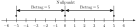
\includegraphics[width=.8\linewidth]{absoluteValue}
 \caption{Der Betrag von sowohl der Zahl 5 als auch der Zahl -5 ist gleich 5.}
 \label{fig:absoluteValue}
 \vspace{.5cm}
\end{figure}

Mathematisch sauber kann man den Betrag so definieren:

\begin{defn}{Betrag einer Zahl}
		Für eine Zahl $a$ ist der Betrag der Zahl
		\[
			|a|=\left\{\begin{array}{ll} a, & a\ge 0 \\
		 -a, & a<0\end{array}\right.
		\]
\end{defn}

\begin{example}
	Vervollständige die Tabelle:\\~\\
	\bgroup
	\def\arraystretch{1.5}
		\begin{tabularx}{\textwidth}{|X||p{2.5em}|p{2.5em}|p{2.5em}|p{2.5em}|p{2.5em}|p{2.5em}|p{2.5em}|p{2.5em}|p{2.5em}|}\hline
			\centering $a$ & \centering $-2$ & \centering $-1.5$ & \centering $-1$ & \centering $-0.5$ & \centering 0 & \centering $0.5$ & \centering 1 & \centering $1.5$ & \hspace{.4cm}2\\\hline
			\centering $|a|$ & & & & & & & & & \\\hline
		\end{tabularx}
	\egroup
\end{example}

\section{Terme}
\subsection*{Auswerten}
Mit $T(a,b)$ bezeichnen wir einen Term, der die Variablen $a$ und $b$ enthält. Setzt man anstelle von $a$ und $b$ Zahlen ein, z.B. 5 für $a$ und 3 für $b$, so schreiben wir $T(5,3)$.
\vspace{1cm}

\subsection*{Termumformungen}
Zwei Terme $T_1$ und $T_2$ heissen \emph{äquivalent (gleichwertig)}, wenn alle möglichen Einsetzungen für die Variable(n) bei $T_1$ denselben Wert ergeben wie bei $T_2$.
Man schreibt: $T_1 = T_2$.
\vspace{5mm}
Einen Term umformen bedeutet:
Man ersetzt ihn durch einen äquivalenten Term. Beim Umformen von Termen werden die arithmetischen Grundgesetze gebraucht.

\begin{law}{Arithmetische Grundgesetze}
    \bgroup
    \def\arraystretch{2.5}
	\begin{tabularx}{\linewidth}{|X|c|c|}
			\hline
			 & Addition & Multiplikation \\
			\hline
			Kommutativgesetz & $a+b=b+a$ & $a\cdot b = b\cdot a$ \\
			
			Assoziativgesetz & $(a+b)+c = a+ (b+c)$ & $(a\cdot b)\cdot c = a\cdot (b\cdot c)$ \\
			
			Es gibt Neutralelement\newline 0 bzw. 1\,. & $a+0 = a$ & $a\cdot 1 = a$ \\
			
			Es gibt inverses Element\newline $-a$ bzw. $\displaystyle \frac{1}{a}$\,. & $a+(-a) = 0$ & $\displaystyle a\cdot \frac{1}{a} = 1$ \\
			\hline
			Distributivgesetz & \multicolumn{2}{c|}{$a(b+c)=ab+ac$} \\
			\hline
    \end{tabularx}
    \egroup
\end{law}

\subsection*{Formeln}
Die \emph{Binomischen Formeln} benutzt man zum schnellen Umformen von Produkten aus Binomen.
Sie stellen Merkformeln dar, die einerseits das Ausmultiplizieren von Klammerausdrücken erleichtern, andererseits aber auch die Faktorisierung von Termen (Umformung von bestimmten Summen und Differenzen in Produkte) erlauben.

\begin{tcolorbox}[colback=blue!7!white,colframe=blue!60!black,title=Binomische Formeln]
	\begin{tabbing}
		$(a+b)^2$ \qquad \, \, \= $=$ \, \= $a^2+2ab+b^2$ \\
		$(a-b)^2$ \qquad \, \, \= $=$ \, \= $a^2-2ab+b^2$ \\
		$(a+b)(a-b)$ \> $=$ \> $a^2-b^2$
	\end{tabbing}
\end{tcolorbox} 

Es gibt auch trinomische Formeln: $(a+b+c)^2$. Kannst du dafür auch einen Ausdruck angeben?
\vspace{2cm}

\subsection*{Erweiterung}
Mit dem \emph{Pascalschen Dreieck} kann man auch höhere Potenzen von Binomen schnell ausmultiplizieren:
\[
	(a+b)^3 =
\]





